\documentclass[12pt]{beamer}
\usepackage{../Estilos/BeamerMAF}
\usepackage{../Estilos/ColoresLatex}
\usetheme{Warsaw}
\usecolortheme{seahorse}
%\useoutertheme{default}
\setbeamercovered{invisible}
% or whatever (possibly just delete it)
\setbeamertemplate{section in toc}[sections numbered]
\setbeamertemplate{subsection in toc}[subsections numbered]
\setbeamertemplate{subsection in toc}{\leavevmode\leftskip=3.2em\rlap{\hskip-2em\inserttocsectionnumber.\inserttocsubsectionnumber}\inserttocsubsection\par}
\setbeamercolor{section in toc}{fg=blue}
\setbeamercolor{subsection in toc}{fg=blue}
\setbeamercolor{frametitle}{fg=blue}
\setbeamertemplate{caption}[numbered]

\setbeamertemplate{footline}
\beamertemplatenavigationsymbolsempty
\setbeamertemplate{headline}{}


\makeatletter
\setbeamercolor{section in foot}{bg=gray!30, fg=black!90!orange}
\setbeamercolor{subsection in foot}{bg=blue!30}
\setbeamercolor{date in foot}{bg=black}
\setbeamertemplate{footline}
{
  \leavevmode%
  \hbox{%
  \begin{beamercolorbox}[wd=.333333\paperwidth,ht=2.25ex,dp=1ex,center]{section in foot}%
    \usebeamerfont{section in foot} \insertsection
  \end{beamercolorbox}%
  \begin{beamercolorbox}[wd=.333333\paperwidth,ht=2.25ex,dp=1ex,center]{subsection in foot}%
    \usebeamerfont{subsection in foot}  \insertsubsection
  \end{beamercolorbox}%
  \begin{beamercolorbox}[wd=.333333\paperwidth,ht=2.25ex,dp=1ex,right]{date in head/foot}%
    \usebeamerfont{date in head/foot} \insertshortdate{} \hspace*{2em}
    \insertframenumber{} / \inserttotalframenumber \hspace*{2ex} 
  \end{beamercolorbox}}%
  \vskip0pt%
}
\makeatother

\makeatletter
\patchcmd{\beamer@sectionintoc}{\vskip1.5em}{\vskip0.8em}{}{}
\makeatother

\newlength{\depthofsumsign}
\setlength{\depthofsumsign}{\depthof{$\sum$}}
\newcommand{\nsum}[1][1.4]{% only for \displaystyle
    \mathop{%
        \raisebox
            {-#1\depthofsumsign+1\depthofsumsign}
            {\scalebox
                {#1}
                {$\displaystyle\sum$}%
            }
    }
}
\def\scaleint#1{\vcenter{\hbox{\scaleto[3ex]{\displaystyle\int}{#1}}}}
\def\scaleoint#1{\vcenter{\hbox{\scaleto[3ex]{\displaystyle\oint}{#1}}}}
\def\bs{\mkern-12mu}


\AtBeginDocument{\RenewCommandCopy\qty\SI}
\ExplSyntaxOn
\msg_redirect_name:nnn { siunitx } { physics-pkg } { none }
\ExplSyntaxOff

\title{\large{2 - Diferenciales y operadores diferenciales}}
\subtitle{Tema 1 - La física y la geometría}

\author{M. en C. Gustavo Contreras Mayén}
\date{}

\begin{document}
\maketitle
\fontsize{14}{14}\selectfont
\spanishdecimal{.}

\section*{Contenido}
\frame[allowframebreaks]{\frametitle{Contenido} \tableofcontents[currentsection, hideallsubsections]}

\section{Diferenciales}
\frame[allowframebreaks]{\frametitle{Temas a revisar} \tableofcontents[currentsection, hideothersubsections]}
\subsection{Diferencial de línea}

\begin{frame}
\frametitle{Construcción}
Utilizando el resultado que define a un vector unitario en un sistema coordenado curvilíneo:
\pause
\begin{align*}
\vu{e}_{i} = \dfrac{1}{h_{i}} \, \pdv{\vb{r}}{u_{i}}
\end{align*}
\pause
para las componentes vectoriales:
\pause
\begin{align*}
\dd{\vb{r}} = \nsum_{i=1}^{3} \pdv{\vb{r}}{u_{i}} \dd{u_{i}}
\end{align*}
\end{frame}
\begin{frame}
\frametitle{Diferencial de línea}
Es posible escribir:
\pause
\begin{align}
\dd{\vb{r}} = \nsum_{i=1}^{3} h_{i} \, \vu{e}_{i} \dd{u_{i}} = \nsum_{i=1}^{3} \dd{\vb{l}_{i}}
\label{eq:ecuacion_01_21}
\end{align}
\pause
donde:
\pause
\begin{align}
\dd{\vb{l}_{i}} = h_{i} \, \vu{e}_{i} \dd{u_{i}}
\label{eq:ecuacion_01_22}
\end{align}
que representa el \textocolor{ao}{elemento diferencial de línea} a lo largo del eje $u_{i}$.
\end{frame}
\begin{frame}
\frametitle{Diferencia de línea}
La ec. (\ref{eq:ecuacion_01_22}) asegura que cualquier elemento de línea con orientación arbitraria, puede descomponerse en una suma vectorial.
\end{frame}

\subsection*{Coordenadas esféricas}

\begin{frame}
\frametitle{Coordenadas esféricas}
En coordenadas esféricas ocupando los factores de escala ya conocidos:
\pause
\begin{align*}
h_{r} & = 1 \\[0.5em]
h_{\theta} & = r \\[0.5em]
h_{\varphi} & = r \, \sin \theta
\end{align*}
\end{frame}
\begin{frame}
\frametitle{Coordenadas esféricas}
Tenemos que:
\pause
\begin{table}
\begin{tabular}{r  c  l}
$\dd{\vb{l}_{r}} = \vu{e}_{r} \dd{r}$ & $\longrightarrow$ & $\dd{l_{r}} = \dd{r}$ \\
$\dd{\vb{l}_{\theta}} = r \, \vu{e}_{\theta} \, \dd{\theta}$ & $\longrightarrow$ & $\dd{l_{\theta}} = r \, \dd{\theta}$ \\
$\dd{\vb{l}_{\varphi}} = r \, \sin \theta \, \vu{e}_{\varphi} \, \dd{\varphi}$ & $\longrightarrow$ & $\dd{l_{\varphi}} = r \, \sin \theta \dd{\varphi}$
\end{tabular}
\end{table}
\end{frame}

\subsection{Diferencial de superficie}

\begin{frame}
\frametitle{Construción}
Las superficies diferenciales se describen como vectores perpendicular al área diferencial, como se ve en la siguiente figura (\ref{fig:figura_diferenciales_superficie}):
\end{frame}
\begin{frame}
\frametitle{Diferenciales de superficie}
\begin{figure}[h!]
    \centering
    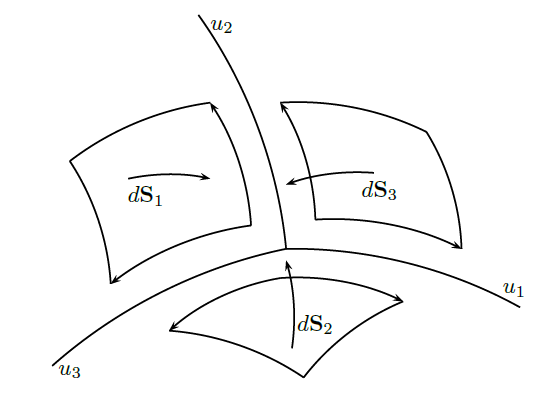
\includegraphics[scale=0.5]{Imagenes/Diferenciales_Superficie_01.png}
    \caption{Elementos diferenciales de área en coordenadas curvilíneas, los vectores mostrados son perpendiculares a su superficie.}
    \label{fig:figura_diferenciales_superficie}
\end{figure}
\end{frame}
\begin{frame}
\frametitle{Diferenciales de superficie}
Las superficies están orientadas según la regla de la mano derecha, por lo que:
\pause
\begin{eqnarray*}
\dd{\vb{S}_{1}} &=& \dd{\vb{l}_{2}} \cp \dd{\vb{l}_{3}} \\[0.5em] \pause
\dd{\vb{S}_{2}} &=& \dd{\vb{l}_{3}} \cp \dd{\vb{l}_{1}} \\[0.5em] \pause
\dd{\vb{S}_{3}} &=& \dd{\vb{l}_{1}} \cp \dd{\vb{l}_{2}}
\end{eqnarray*}
\end{frame}
\begin{frame}
\frametitle{Usando un resultado previo}
Usando las relaciones:
\pause
\begin{align*}
\vu{e}_{1} \cp \vu{e}_{2} = \vu{e}_{3} \\
\vu{e}_{2} \cp \vu{e}_{3} = \vu{e}_{1} \\
\vu{e}_{3} \cp \vu{e}_{1} = \vu{e}_{2}
\end{align*}
que son válidas para sistemas coordenados curvilíneos ortonormales, en espacios 3D euclidianos.
\end{frame}
\begin{frame}
\frametitle{Usando un resultado previo}
Que en forma sintética queda expresado por:
\pause
\begin{align}
\vu{e}_{i} \cp \vu{e}_{j} = \nsum_{i=1}^{3} \epsilon_{ijk} \, \vu{e}_{k}
\end{align}
donde $\epsilon_{ijk}$ es el símbolo de \emph{Levi-Civita} que definimos en la presentación anterior.
\end{frame}
\begin{frame}
\frametitle{Diferenciales de superficie}
Así encontramos que:
\pause
\begin{eqnarray*}
\begin{aligned}
\dd{\vb{S}_{1}} &= \left( h_{2} \, \vu{e}_{2} \, \dd{u}_{2} \right) \cp \left( h_{3} \, \vu{e}_{3} \, \dd{u}_{3} \right) = \\[0.5em] \pause
&= \left( \vu{e}_{2} \cp \vu{e}_{3} \right) \, h_{2} \, h_{3} \, \dd{u_{2}} \dd{u_{3}} = \\[0.5em] \pause
&= \vu{e}_{1} \, h_{2} \, h_{3} \, \dd{u_{2}} \, \dd{u_{3}} = \\[0.5em] \pause
&= \vu{e}_{1} \dd{S_{1}}
\end{aligned}
\end{eqnarray*}
\end{frame}
\begin{frame}
\frametitle{Superficies diferenciales}
Para el otro diferencial de superficie:
\pause
\begin{eqnarray*}
\begin{aligned}
\dd{\vb{S}_{2}} &= \left( h_{3} \, \vu{e}_{3} \, \dd{u}_{3} \right) \cp \left( h_{1} \, \vu{e}_{1} \, \dd{u}_{1} \right) = \\[0.5em]
&= \left( \vu{e}_{3} \cp \vu{e}_{1} \right) \, h_{3} \, h_{1} \, \dd{u_{3}} \dd{u_{1}} = \\[0.5em]
&= \vu{e}_{2} \, h_{3} \, h_{1} \, \dd{u_{3}} \dd{u_{1}} = \\[0.5em]
&= \vu{e}_{2} \dd{S_{2}}
\end{aligned}
\end{eqnarray*}
\end{frame}
\begin{frame}
\frametitle{Superficies diferenciales}
Y por último:
\begin{eqnarray*}
\begin{aligned}    
\dd{\vb{S}_{3}} &= \left( h_{1} \, \vu{e}_{1} \, \dd{u}_{1} \right) \cp \left( h_{2} \, \vu{e}_{2} \, \dd{u}_{2} \right) = \\[0.5em]
&= \left( \vu{e}_{1} \cp \vu{e}_{2} \right) \, h_{1} \, h_{2} \, \dd{u_{1}} \dd{u_{2}} = \\[0.5em]
&= \vu{e}_{3} \, h_{1} \, h_{2} \, \dd{u_{1}} \dd{u_{2}} = \\[0.5em]
&= \vu{e}_{3} \dd{S_{3}}
\end{aligned}
\end{eqnarray*}
\end{frame}

\subsection{Diferencial de volumen}

\begin{frame}
\frametitle{Construcción de un elemento de volumen}
El elemento diferencial de volumen se define como:
\pause
\begin{eqnarray*}
\begin{aligned}
\dd{V} &= \dd{\vb{l}_{1}} \cdot \dd{\vb{l}_{2}} \cp \dd{\vb{l}_{3}} = \\ \pause
&= \left( h_{1} \, \vu{e}_{1} \, \dd{u}_{1} \right) \vdot \left( h_{2} \, \vu{e}_{2} \, \dd{u}_{2} \right) \cp \left( h_{3} \, \vu{e}_{3} \, \dd{u}_{3} \right) =  \\[0.5em]
&= \left( \vu{e}_{1} \cdot \vu{e}_{2} \cp \vu{e}_{3} \right) \, h_{1} \, h_{2} \, h_{3} \, \dd{u_{1}} \dd{u_{2}} \dd{u_{3}} = \\ \pause
&= h_{1} \, h_{2} \, h_{3} \dd{u_{1}} \dd{u_{2}} \dd{u_{3}}
\end{aligned}
\end{eqnarray*}
\end{frame}

\subsection*{Coordenadas esféricas}

\begin{frame}
\frametitle{Coordenadas esféricas}
En coordenadas esféricas tenemos:
\pause
\begin{eqnarray*}
\dd{S_{1}} &=& \dd{S_{r}} = h_{\theta} \, h_{\varphi} \dd{\theta} \dd{\varphi} = r^{2} \sin \theta \dd{\theta} \dd{\varphi} \\[0.5em] \pause
\dd{S_{2}} &=& \dd{S_{\theta}} = h_{\varphi} \, h_{r} \dd{\varphi} \dd{r} = r \sin \theta \dd{r} \dd{\varphi} \\[0.5em] \pause
\dd{S_{3}} &=& \dd{S_{\varphi}} = h_{r} \, h_{\theta} \dd{r} \dd{\theta} = r \dd{r} \dd{\theta}
\end{eqnarray*}
\end{frame}
\begin{frame}
\frametitle{Construcción del elemento de volumen}
Entonces el diferencial de volumen es:
\pause
\begin{eqnarray*}
\dd{V} &=& h_{r} \, h_{\theta} \, h_{\varphi} \dd{r} \dd{\theta} \dd{\varphi} = \\[0.5em] \pause
&=& r^{2} \, \sin \theta \dd{r} \dd{\theta} \dd{\varphi}
\end{eqnarray*}
\end{frame}
\begin{frame}
\frametitle{Ejercicio a cuenta}
La velocidad y la aceleración se definen en la forma vectorial como:
\begin{align*}
\vb{v} = \dv{\vb{r}}{t} = \dot{\vb{r}} \hspace{1cm} \vb{a} = \dot{\vb{v}} = \ddot{\vb{r}}
\end{align*}
Calcula para el sistema coordenado esférico:
\setbeamercolor{item projected}{bg=denim,fg=white}
\setbeamertemplate{enumerate items}{%
\usebeamercolor[bg]{item projected}%
\raisebox{1.5pt}{\colorbox{bg}{\color{fg}\footnotesize\insertenumlabel}}%
}
\begin{enumerate}[<+->]
\item $\dot{\vu{e}}_{r}$, $\dot{\vu{e}}_{\theta}$, $\dot{\vu{e}}_{\varphi}$ 
\item La velocidad: $\vb{v}$
\item La aceleración: $\vb{a}$
\end{enumerate}
\end{frame}
% \begin{frame}
% \frametitle{Ejercicio a cuenta}
% Demuestra que para dos vectores $\vb{A}$ y $\vb{B}$:
% \setbeamercolor{item projected}{bg=blue!70!black,fg=yellow}
% \setbeamertemplate{enumerate items}[circle]
% \begin{enumerate}
% \item $\vb{A} \cp \vb{B} = \displaystyle \nsum_{ijk} \, \vu{e}_{i} \, \epsilon_{ijk} \, A_{j} \, B_{k}$ \\[1em]
% \item $\vb{A} \cdot \vb{B} \cp \vb{C} = \displaystyle \nsum_{ijk} \, \epsilon_{ijk} \, A_{i} \, B_{j} \, C_{k}$
% \end{enumerate}
% \end{frame}

\section{Operadores diferenciales}
\frame[allowframebreaks]{\frametitle{Temas a revisar} \tableofcontents[currentsection, hideothersubsections]}
\subsection{Características de los campos}

\begin{frame}
\frametitle{Sobre los campos escalares y vectoriales}
En la presentación anterior mencionamos la naturaleza de los campos escalares y vectoriales.
\\
\bigskip
\pause
Asumiremos que los campos son funciones regulares, continuas y derivables, excepto posiblemente en algunos puntos aislados.
\end{frame}
\begin{frame}
\frametitle{Sobre los campos escalares y vectoriales}
En general los campos serán descritos por ecuaciones diferenciales parciales cuyas variables independientes serán la posición y el tiempo.
\end{frame}

\section{Gradiente}
\frame[allowframebreaks]{\frametitle{Temas a revisar} \tableofcontents[currentsection, hideothersubsections]}
\subsection{Definición}

\begin{frame}
\frametitle{El gradiente}
Al pasar de un punto:
\pause
\begin{align*}
P (u_{1}, u_{2}, u_{3})
\end{align*}
\pause
a otro infinitesimalmente cercano:
\pause
\begin{align*}
P (u_{1} + \dd{u}_{1}, u_{2} + \dd{u_{2}} + u_{3} + \dd{u_{3}})
\end{align*}
\end{frame}
\begin{frame}
\frametitle{El gradiente}
El cambio diferencial de una función (o campo) escalar $\phi(u_{1}, u_{2}, u_{3})$ está dado por:
\pause
\begin{align}
\begin{aligned}[b]
\dd{\phi} &= \pdv{\phi}{u_{1}} \dd{u_{1}} + \pdv{\phi}{u_{2}} \dd{u_{2}} + \pdv{\phi}{u_{3}} \dd{u_{3}} = \\[0.5em]
&= \nsum_{i=1}^{3} \pdv{\phi}{u_{i}} \dd{u_{i}}
\end{aligned}
\label{eq:ecuacion_01_26}
\end{align}
\end{frame}
\begin{frame}
\frametitle{El gradiente}
Teniendo en cuenta la ec. (\ref{eq:ecuacion_01_21}) se sigue que:
\pause
\begin{align}
\dd{\vb{r}} = \nsum_{j=1}^{3} h_{j} \, \vu{e}_{j} \dd{u_{j}}
\label{eq:ecuacion_01_27}
\end{align}
\pause
Multiplicando escalarmente por $\vu{e}_{i}$ tenemos que:
\end{frame}
\begin{frame}
\frametitle{El gradiente}
\begin{eqnarray*}
\begin{aligned}
\dd{\vb{r}} \vdot \vu{e}_{i} &= \left( \nsum_{j=1}^{3} h_{j} \, \vu{e}_{j} \dd{u_{j}} \right) \vdot \vu{e}_{i} = \\[0.5em] \pause
&= \nsum_{j=1}^{3} \left( \vu{e}_{j} \cdot \vu{e}_{i} \right) \, h_{j} \, \dd{u_{j}} = \pause \nsum_{j=1}^{3} \delta_{ij} \, h_{j} \, \dd{u_{j}} = \\[0.5em] \pause
&= h_{i} \dd{u_{i}} \\[1em] \pause
&\Longrightarrow \dd{u_{i}} = \dfrac{1}{h_{i}} \dd{\vb{r}} \cdot \vu{e}_{i}
\end{aligned}
\end{eqnarray*}
\end{frame}
\begin{frame}
\frametitle{El gradiente}
Al sustituir en la ec. (\ref{eq:ecuacion_01_26}), llegamos a:
\pause
\begin{eqnarray*}
\begin{aligned}
\dd{\phi} &= \nsum_{i=1}^{3} \pdv{\phi}{u_{i}} \, \dfrac{1}{h_{i}} \, \vu{e}_{i} \cdot \dd{\vb{r}} = \\[0.5em] \pause
&= \dd{\vb{r}} \cdot \left( \nsum_{i=1}^{3} \dfrac{\vu{e_{i}}}{h_{i}} \, \pdv{\phi}{u_{i}} \right)
\end{aligned}
\end{eqnarray*}
\pause
Al término entre paréntesis lo denotamos $\grad{\phi}$.
\end{frame}
\begin{frame}
\frametitle{Definición del gradiente}
El operador \textocolor{cobalt}{nabla} (también conocido como \textocolor{coquelicot}{del}) es:
\pause
\begin{align}
\grad{\phi} = \nsum_{i=1}^{3} \dfrac{\vu{e_{i}}}{h_{i}} \, \pdv{\phi}{u_{i}} = \nsum_{i=1}^{3} \vu{e}_{i} \left( \grad{\phi} \right)_{i}
\label{eq:ecuacion_01_28}
\end{align}
\pause
Se le llamará \textocolor{armygreen}{gradiente de la función escalar} $\phi(u_{i})$, por tanto:
\pause
\begin{align}
\dd{\phi} = \dd{\vb{r}} \cdot \grad{\phi}
\label{eq:ecuacion_01_29}
\end{align}
\end{frame}
\begin{frame}
\frametitle{Derivada direccional}
Como tenemos que:
\pause
\begin{align*}
\dd{\vb{r}} = \vu{n} \dd{l}
\end{align*}
\pause
Se sigue que:
\pause
\begin{align*}
\dv{\phi}{l} = \vu{n} \cdot \grad{\phi}
\end{align*}
que corresponde a la definición de \textocolor{blue}{derivada direccional} de la función $\phi$ en la dirección de $\vu{n}$.
\end{frame}

\subsection{Propiedades del gradiente}

\begin{frame}
\frametitle{Superficies cercanas}
Para estudiar las propiedades del gradiente tomemos un par de superficies infinitesimalmente cercanas, sobre cada una de las cuales la función $\phi$ toma valores constantes e infinitesimalmente distintos: $\phi$ y $\phi + \dd{\phi}$.
\\
\bigskip
\pause
En la teoría de campos se les llama \textocolor{awesome}{superficies equipotenciales}.
\end{frame}
\begin{frame}
\frametitle{Superficies equipotenciales}
\begin{figure}[h!]
    \centering
    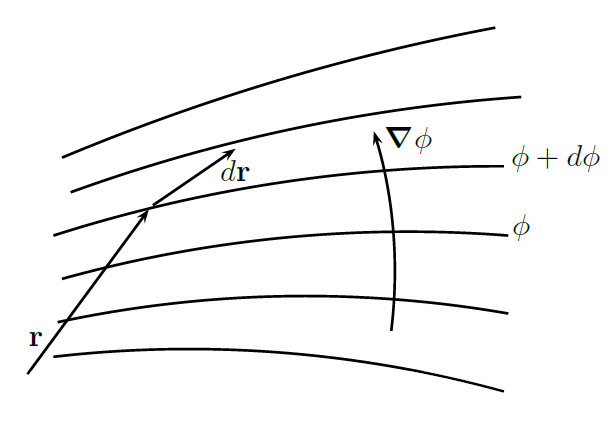
\includegraphics[scale=0.5]{Imagenes/Superficies_Equipotenciales.png}
    \caption{Superficies equipotenciales.}
    \label{fig:Superficies_Equipotenciales}
\end{figure}
\end{frame}
\begin{frame}
\frametitle{Propiedades del gradiente}
De la ec. (\ref{eq:ecuacion_01_29}) se tiene que:
\pause
\begin{align*}
\dd{\phi} = \dd{\vb{r}} \cdot \grad{\phi} = \abs{\dd{\vb{r}}} \, \abs{\grad{\phi}} \, \cos \theta
\end{align*}
donde $\theta$ es el ángulo entre $\dd{\vb{r}}$ y $\grad{\phi}$.
\end{frame}
\begin{frame}
\frametitle{Propiedades del gradiente}
Si el vector $\dd{\vb{r}}$ se sitúa en el plano $\phi = \text{ constante}$, entonces: $\dd{\phi} = 0$, por lo que:
\pause
\begin{align*}
0 = \abs{\dd{\vb{r}}} \, \abs{\grad{\phi}} \, \cos \theta
\end{align*}
\pause
Como $\grad{\phi}$ es en general diferente de cero, ya que $\phi(u_{i})$ es una función arbitraria, y como $\abs{\dd{\vb{r}}} \neq 0$, se sigue que $\cos \theta = 0$, entonces $\theta = \ang{90}$
\end{frame}
\begin{frame}
\frametitle{Propiedades del gradiente}
En consecuencia: $\grad{\phi}$ es \textocolor{debianred}{perpendicular} a la superficie $\phi = \text{ constante}$.
\\
\bigskip
\pause
El valor máximo de $\dd{\phi}$ se presenta cuando $\theta = 0$, es decir:
\pause
\begin{eqnarray*}
\begin{aligned}
\dd{\phi}_{\max} = \abs{\grad{\phi}} \, \abs{\dd{\vb{r}}} &= \abs{\grad{\phi}} \dd{l} \\[1em] \pause
\text{o cuando } \hspace{0.5cm} \left( \dv{\phi}{l} \right)_{\max} &= \abs{\grad{\phi}}
\end{aligned}
\end{eqnarray*}
\end{frame}
\begin{frame}
\frametitle{Módulo del gradiente}
Entonces el módulo del gradiente corresponde al valor máximo de la derivada direccional y el gradiente apunta en la dirección en que tal derivada es máxima.
\end{frame}
\begin{frame}
\frametitle{Construcción de sistema curvilíneos}
Dado que para cada punto de una línea o superficie equipotencial es posible trazar el vector $\grad{\phi}$, entonces es posible construir una red coordenada ortogonal a las equipotenciales.
\end{frame}
\begin{frame}
\frametitle{Construcción de sistema curvilíneos}
Por lo que, dada una familia de curvas en el plano (o de superficies curvas en el espacio), es posible obtener otras que le sean ortogonales.
\end{frame}
\begin{frame}
\frametitle{Construcción de sistema curvilíneos}
Por lo que tenemos un método eficaz de construcción de sistemas de coordenadas curvilíneas ortogonales.
\end{frame}
\begin{frame}
\frametitle{Consideración importante}
Hay que tomar en cuenta que $\grad$ \emph{no} es un vector, sino un \textbf{operador vectorial}: $\grad$ no tiene dirección, a menos que opere sobre una función.
\end{frame}
\begin{frame}
\frametitle{Ejercicios a cuenta}
Para ejercitar el avance que llevamos, resuelve:
\setbeamercolor{item projected}{bg=lava,fg=white}
\setbeamertemplate{enumerate items}{%
\usebeamercolor[bg]{item projected}%
\raisebox{1.5pt}{\colorbox{bg}{\color{fg}\footnotesize\insertenumlabel}}%
}
\begin{enumerate}
\item Demuestra que $\grad{\left( \phi \psi \right)} = \phi \, \grad{\psi} + \psi \, \grad{\phi}$
\item Si $f = f(r)$ con $r = \sqrt{x^{2} + y^{2}+ z^{2}}$, demuestra que
\begin{align*}
\nabla{f(r)} = \vu{r} \, \dv{f(r)}{r}
\end{align*}
\end{enumerate}
\end{frame}

\section{Divergencia}
\frame[allowframebreaks]{\frametitle{Temas a revisar} \tableofcontents[currentsection, hideothersubsections]}
\subsection{Flujo de campo vectorial}

\begin{frame}
\frametitle{Flujo de campo vectorial}
Dada una superficie diferencial orientada $\dd{\vb{S}}$ (figura \ref{fig:figura_superficie_diferencial}), se define el \emph{flujo} del campo vectorial $\vb{B}$ a través de $\dd{\vb{S}}$ como:
\pause
\begin{align*}
\mbox{flujo diferencial } = \dd{\Phi} = \vb{B} \cdot \dd{\vb{S}}
\end{align*}
\end{frame}
\begin{frame}
\frametitle{Superficie diferencial}
\begin{minipage}{0.45\linewidth}
\begin{figure}[h!]
    \centering
    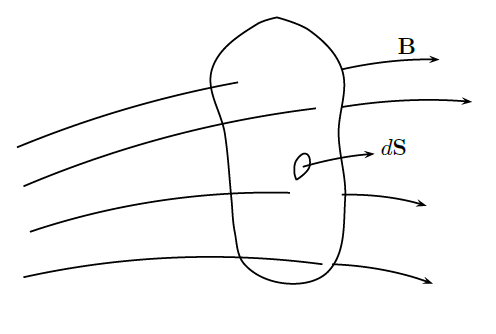
\includegraphics[scale=0.35]{Imagenes/Superficie_Diferencial.png}
    \caption{Flujo del campo $\vb{B}$ a través de una superficie abierta.}
    \label{fig:figura_superficie_diferencial}
\end{figure}
\end{minipage}
\hspace{1cm}
\pause
\begin{minipage}{0.4\linewidth}
\fontsize{12}{12} \selectfont
El flujo es máximo si \\ $\vb{B} \parallel \dd{\vb{S}}$ y es nulo si $\vb{B} \bot \dd{\vb{S}}$.
\end{minipage}
\end{frame}
\begin{frame}
\frametitle{Superficie diferencial cerrada}
Nos enfocaremos en el cálculo del flujo a través de una superficie diferencial \emph{cerrada}, que contenga un volumen diferencial $\dd{V}$ limitado por superficies coordenadas.
\end{frame}
\begin{frame}
\frametitle{Superficie diferencial cerrada}
El volumen será entonces un paralelepípedo curvilíneo:
\begin{figure}[h!]
    \centering
    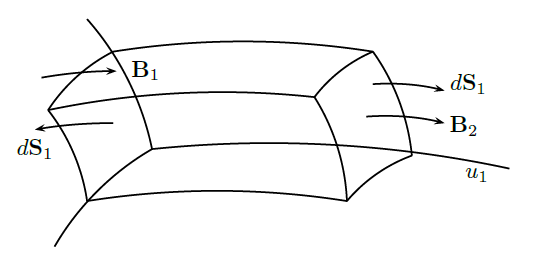
\includegraphics[scale=0.5]{Imagenes/Diferencial_Volumen.png}
    \caption{Elemento diferencial de volumen.}
    \label{fig:Diferencial_Volumen}
\end{figure}
\end{frame}
\begin{frame}
\frametitle{Flujo total en una cara}
Consideraremos el flujo total como la suma de los flujos a través de cada pareja de superficies.
\\
\bigskip
\pause
Como primer paso, analizamos el flujo sobre las caras $\dd{\vb{S}_{1}}$:
\end{frame}
\begin{frame}
\frametitle{Flujo total en un cara}
El flujo sobre las caras $\dd{\vb{S}_{1}}$:
\pause
\begin{eqnarray*}
\begin{aligned}
&\dd{\Phi} = \dd{\Phi_{u_{1} + \dd{u_{1}}}} + \dd{\Phi_{u_{1}}} \\[0.5em] \pause
&= \left( B_{1} \dd{S_{1}} \right)_{u_{1} + \dd{u_{1}}} - \left( B_{1} \dd{S_{1}} \right)_{u_{1}} \\[0.5em] \pause
&= \left( B_{1} \, h_{2} \, h_{3} \dd{u_{2}} \dd{u_{3}} \right)_{u_{1} + \dd{u_{1}}} - \left( B_{1} \, h_{2} \, h_{3} \dd{u_{2}} \dd{u_{3}} \right)_{u_{1}} \\[0.5em] \pause
&= \left( B_{1} \, h_{2} \, h_{3} \right)_{u_{1} + \dd{u_{1}}} \dd{u_{2}} \dd{u_{3}} - \left( B_{1} \, h_{2} \, h_{3} \right)_{u_{1}} \dd{u_{2}} \dd{u_{3}}
\end{aligned}
\end{eqnarray*}
\end{frame} 
\begin{frame}
\frametitle{Elementos diferenciales}
Los elementos diferenciales $\dd{u_{2}} \dd{u_{3}}$ han sido extraídos del primer término, ya que son independientes de $u_{1}$.
\end{frame}
\begin{frame}
\frametitle{Expansión en serie de Taylor}
Si hacemos una expansión en serie de Taylor alrededor de $u_{1}$, tendremos:
\pause
\begin{align*}
\left( B_{1} \, h_{2} \, h_{3} \right)_{u_{1} + \dd{u_{1}}} &= \left( B_{1} \, h_{2} \, h_{3} \right)_{u_{1}} + \\[0.5em]
&+ \pdv{\left( B_{1} \, h_{2} \, h_{3} \right)}{u_{1}} \dd{u_{1}} + \ldots
\end{align*}
\end{frame}
\begin{frame}
\frametitle{Flujo sobre una cara}
Por lo que el flujo sobre una cara resulta:
\pause
\begin{eqnarray*}
\dd{\Phi_{1}} &=& \pdv{\left( B_{1} \, h_{2} \, h_{3} \right)}{u_{1}} \dd{u_{1}} \dd{u_{2}} \dd{u_{3}} = \\[0.5em] \pause
&=& \pdv{\left( B_{1} \, h_{2} \, h_{3} \right)}{u_{1}} \, \dfrac{\dd{V}}{h_{1} h_{2} h_{3}}
\end{eqnarray*}
\end{frame}
\begin{frame}
\frametitle{Flujo en las otras caras}
De manera análoga, el flujo en las otras caras es:
\pause
\begin{align*}
\dd{\Phi_{2}} &= \pdv{\left( B_{2} \, h_{3} \, h_{1} \right)}{u_{2}} \, \dfrac{\dd{V}}{h_{1} h_{2} h_{3}} \\[1em]
\dd{\Phi_{3}} &= \pdv{\left( B_{3} \, h_{1} \, h_{2} \right)}{u_{3}} \, \dfrac{\dd{V}}{h_{1} h_{2} h_{3}}
\end{align*}
\end{frame}
\begin{frame}
\frametitle{Flujo total}
El flujo total $\dd{\Phi}$ que atraviesa el volumen $\dd{V}$ es:
\pause
\begin{align*}
&\dd{\Phi} = \dd{\Phi_{1}} + \dd{\Phi_{2}} + \dd{\Phi_{3}} = \\[1em]
&= \left[ \pdv{\left( B_{1} \, h_{2} \, h_{3} \right)}{u_{1}} + \pdv{\left( B_{2} \, h_{3} \, h_{1} \right)}{u_{2}} + \right. \\[0.5em] 
&+ \left.  \pdv{\left( B_{3} \, h_{1} \, h_{2} \right)}{u_{3}} \right] \, \dfrac{\dd{V}}{h_{1} h_{2} h_{3}}
\end{align*}
\end{frame}
\begin{frame}
\frametitle{Flujo total simplificado}
Hacemos $h \equiv h_{1} h_{2} h_{3}$, por lo que el flujo total es:
\pause
\begin{align*}
\dd{\Phi} &= \left[ \pdv{u_{1}} \left( \dfrac{B_{1} \, h}{h_{1}} \right) + \pdv{u_{2}} \left( \dfrac{B_{2} \, h}{h_{2}} \right) + \right. \\[0.5em]
&+ \left. \pdv{u_{3}} \left( \dfrac{B_{3} \, h}{h_{3}} \right) \right] = \\[1em]
&= {\rm Div} \, \vb{B} \dd{V}
\end{align*}
\end{frame}

\subsection{Definición de divergencia}

\begin{frame}
\frametitle{Definición de divergencia}
Se define la \emph{divergencia del campo $\vb{B}$} como la siguiente función escalar:
\pause
\begin{align}
{\rm Div} \, \vb{B} = \dfrac{1}{h} \nsum_{i=1}^{3} \pdv{u_{i}} \left( \dfrac{B_{i} \, h}{h_{i}} \right)
\label{eq:ecuacion_01_30}
\end{align}
\end{frame}
\begin{frame}
\frametitle{La divergencia}
La divergencia es el \textocolor{carmine}{flujo por unidad de volumen}:
\begin{align*}
{\rm Div} \, \vb{B} = \dfrac{\dd{\Phi}}{\dd{V}}
\end{align*}
\pause
Este resultado se ha obtenido para una unidad de volumen diferencial.
\end{frame}
\begin{frame}
\frametitle{Flujo para un volumen finito}
Para un volumen finito tenemos que:
\pause
\begin{align*}
\Phi = \oint \vb{B} \cdot \dd{\vb{S}}
\end{align*}
donde ya sabemos que la integración se realiza sobre una superficie \textbf{cerrada}.
\end{frame}
\begin{frame}
\frametitle{Cálculo de la integral}
Para calcular la integral cerrada (que equivale a sumar flujos diferenciales), se descompone el volumen $V$ en un conjunto de volúmenes diferenciales $\dd{V}$.
\end{frame}
\begin{frame}
\frametitle{Cálculo de la integral}
Las caras comunes de los paralelepípedos diferenciales contribuyen con flujos iguales y opuestos en signo, que se cancelan al hacer la suma.
\\
\bigskip
\pause
Las partes no nulas de la integral de área son aquellas que corresponden a caras de la frontera.
\end{frame}
\begin{frame}
\frametitle{Cálculo de la integral}
Por lo que:
\pause
\begin{align*}
\Phi = \scaleoint{6ex} \vb{B} \cdot \dd{\vb{S}} = \scaleint{6ex} {\rm Div} \, \vb{B} \dd{V}
\end{align*}
\pause
La integral de la divergencia sobre un volumen puede transformarse en una integral que involucra sólo el valor del campo sobre la superficie.
\end{frame}

\subsection{Teorema de la divergencia}

\begin{frame}
\frametitle{Teorema de la divergencia}
El resultado anterior se conoce como el \textocolor{cadetblue}{Teorema de la divergencia}:
\pause
\begin{align}
\scaleoint{6ex} \vb{B} \cdot \dd{\vb{S}} = \scaleint{6ex} {\rm Div} \, \vb{B} \dd{V}
\label{eq:ecuacion_01_31}
\end{align}
La integral se extiende sobre la superficie que rodea al volumen $V$.
\end{frame}
\begin{frame}
\frametitle{Otra expresión para la divergencia}
De modo alterno tenemos que:
\pause
\begin{align*}
{\rm Div} \, \vb{B} = \lim_{\Delta V \to 0} \dfrac{\displaystyle \scaleoint{6ex} \vb{S} \dd{\vb{S}}}{\Delta V}
\end{align*}
\end{frame}
\begin{frame}
\frametitle{Divergencia en coordenadas curvilíneas}
En coordenadas curvilíneas ortogonales se tiene que:
\pause
\begin{align*}
{\rm Div} \, \vb{B} = \div{\vb{B}}
\end{align*}
\pause
El lado izquierdo de la igualdad se calcula con la ec. (\ref{eq:ecuacion_01_30}) y el lado derecho utilizando el operador gradiente de la ec. (\ref{eq:ecuacion_01_28}).
\end{frame}
\begin{frame}
\frametitle{Ejercicio a cuenta}
Demuestra que el campo eléctrico de una carga puntal
\begin{align*}
\vb{E} = \dfrac{q \, \vu{r}}{4 \, \pi \epsilon_{0} \, r^{2}}
\end{align*}
cumple $\div{E} = 0$, para $r \neq 0$.
\end{frame}
% \begin{frame}
% \frametitle{Ejercicio a cuenta}
% La ley de Gauss para el campo eléctrico tiene la forma:
% \begin{align*}
% \oint \vb{E} \cdot \dd{\vb{S}} = \dfrac{q}{\epsilon_{0}}
% \end{align*}
% donde $q = \displaystyle \int \rho \dd{V}$ es la carga encerrada en la superficie y $\rho$ su densidad volumétrica.
% \\
% \bigskip
% Demuestra la ley de Gauss en forma diferencial
% \begin{align*}
% \div{E} = \dfrac{\rho}{\epsilon_{0}}
% \end{align*}
% \end{frame}

\section{Rotacional}
\frame[allowframebreaks]{\frametitle{Temas a revisar} \tableofcontents[currentsection, hideothersubsections]}
\subsection{Circulación de un vector}

\begin{frame}
\frametitle{Circulación de un vector}
Se define la \textocolor{byzantine}{circulación} de un vector a lo largo de una curva cerrada como:
\pause
\begin{align*}
\scaleoint{6ex} \vb{B} \cdot \dd{\vb{l}}
\end{align*}
\pause
\begin{figure}[h!]
    \centering
    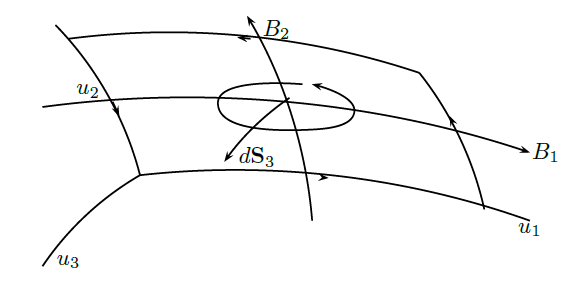
\includegraphics[scale=0.4]{Imagenes/Circulacion_Vector.png}
    \caption{Trayectoria cerrada sobre la superficie $u_{1} \, u_{3}$}
    \label{fig:figura_trayectoria_cerrada}
\end{figure}
\end{frame}
\begin{frame}
\frametitle{Circuito diferencial}
Para el circuito diferencial de la figura (\ref{fig:figura_trayectoria_cerrada}):
\pause
\begin{align*}
\scaleoint{6ex}_{3} \vb{B} \cdot \dd{\vb{l}} &= - \left( B_{2} \dd{l_{2}} \right)_{u_{1}} + \left( B_{1} \dd{l_{1}} \right)_{u_{2}} + \\[0.5em]
&+ \left( B_{2} \dd{l_{2}} \right)_{u_{1}+\dd{u_{1}}} - \left( B_{1} \dd{l_{1}} \right)_{u_{2}+\dd{u_{2}}}
\end{align*}
\end{frame}
\begin{frame}
\frametitle{Expandiendo en una serie}
Como en el caso de la divergencia, expandimos en una serie de Taylor para luego cancelar términos:
\pause
\begin{eqnarray*}
\begin{aligned}
\scaleoint{6ex}_{3} \vb{B} \cdot \dd{\vb{l}} &= \left[ \displaystyle \pdv{u_{1}} \left( B_{2} \, h_{2}\right) - \pdv{u_{2}} \left( B_{1} \, h_{1} \right) \right] \dd{u_{1}} \dd_{u_{2}} = \\[0.5em] \pause
&= \left[ \pdv{u_{1}} \left( B_{2} \, h_{2}\right) - \pdv{u_{2}} \left( B_{1} \, h_{1} \right) \right] \, \dfrac{\dd{S_{3}}}{h_{1} h_{2}} = \\[0.5em] \pause
&= ({\rm{Rot}} \, \vb{B})_{3} \dd{S_{3}}
\end{aligned}
\end{eqnarray*}
\end{frame}
\begin{frame}
\frametitle{Cálculo para las otras dos superficies}
El cálculo realizado ha sido considerando sólo la superficie $\dd{S_{3}}$, por lo que hay que incluir las trayectorias sobre las superficies $u_{1} = \text{cte.}$ y $u_{2} = \text{cte.}$, así tendremos:
\end{frame}
\begin{frame}
\frametitle{Cálculo para las otras dos superficies}
Entonces:
\pause
\begin{align*}
\scaleoint{6ex}_{\bs 1} \vb{B} \cdot \dd{\vb{l}} &= ({\rm{Rot}} \, \vb{B})_{1} \dd{S_{1}} \\[1em]
\scaleoint{6ex}_{\bs 2} \vb{B} \cdot \dd{\vb{l}} &= ({\rm{Rot}} \, \vb{B})_{2} \dd{S_{2}}
\end{align*}
\end{frame}
\begin{frame}
\frametitle{El cálculo para una curva cerrada}
Los resultados anteriores consideran solo a los paralelogramos curvilíneos localizados en las superficies coordenadas.
\\
\bigskip
\pause
El caso general se presenta con la curva cerrada $c$ en el espacio, que rodea una superficie diferencial $\dd{\vb{S}}$.
\end{frame}
\begin{frame}
\frametitle{El cálculo para una curva cerrada}
La curva cerrada se puede descomponer en $\dd{S_{1}}$, $\dd{S_{2}}$, $\dd{S_{3}}$, entonces:
\pause
\begin{align*}
\scaleoint{6ex}_{c} \vb{B} \cdot \dd{\vb{l}} = ({\rm{Rot}} \, \vb{B})_{1} \cdot \dd{S} 
\end{align*}
\end{frame}

\subsection{Definición del rotacional}

\begin{frame}
\frametitle{El rotacional}
Entonces llegamos a:
\pause
\begin{align*}
{\rm Rot} \, \vb{B} &= \dfrac{\vu{e}_{1}}{h_{2} h_{3}} \left[ \displaystyle \pdv{u_{2}} \left( B_{3} \, h_{3} \right) - \pdv{u_{3}} \left( B_{2} \, h_{2} \right) \right] + \\[0.5em]
&+ \dfrac{\vu{e}_{2}}{h_{3} h_{1}} \left[ \displaystyle \pdv{u_{3}} \left( B_{1} \, h_{1} \right) - \pdv{u_{1}} \left( B_{3} \, h_{3} \right) \right] + \\[0.5em]
&+ \dfrac{\vu{e}_{3}}{h_{1} h_{2}} \left[ \displaystyle \pdv{u_{1}} \left( B_{2} \, h_{2} \right) - \pdv{u_{2}} \left( B_{1} \, h_{1} \right) \right]
\end{align*}
\end{frame}
\begin{frame}
\frametitle{El rotacional}
Ocupando el símbolo de Levi-Civita y con $h = h_{1} \, h_{2} \, h_{3}$, tenemos:
\pause
\begin{align}
\begin{aligned}[b]
{\rm Rot} \, \vb{B} &= \dfrac{1}{h} \nsum_{i,j,k=1}^{3} \vu{e}_{i} \, \epsilon_{ijk} \, h_{i} \, \pdv{u_{j}} \left( B_{k} \, h_{k} \right) = \\[1em]
&= \nsum_{i=1}^{3} \vu{e}_{i} \left( {\rm Rot} \, \vb{B} \right)_{i}
\end{aligned}
\label{eq:ecuacion_01_34}
\end{align}
\end{frame}
\begin{frame}
\frametitle{Forma matricial del rotacional}
En forma matricial queda expresado como:
\pause
\begin{align*}
{\rm Rot} \, \vb{B} = \dfrac{1}{h_{1} h_{2} h_{3}}\mdet{
h_{1} \, \vu{e}_{1} & h_{2} \, \vu{e}_{2} & h_{3} \, \vu{e}_{3} \\
\displaystyle \pdv{u_{1}} & \displaystyle \pdv{u_{2}} & \displaystyle \pdv{u_{3}} \\
B_{1} \, h_{1} & B_{2} \, h_{2} & B_{3} \, h_{3}
}
\end{align*}
El operador $\pdv*{u_{i}}$ opera solo sobre la tercera fila.
\end{frame}
\begin{frame}
\frametitle{Resultado importante}
Es posible demostrar que:
\pause
\begin{align*}
{\rm Rot} \, \vb{B} = \curl{B}
\end{align*}
\end{frame}
\begin{frame}
\frametitle{Otro resultado importante}
De la expresión:
\pause
\begin{align*}
\scaleoint{6ex}_{c} \vb{B} \cdot \dd{\vb{l}} = (\curl{\vb{B}}) \cdot \dd{\vb{S}}
\end{align*}
\pause
se sigue que:
\pause
\begin{align*}
\scaleoint{6ex} \vb{B} \cdot \dd{\vb{l}} = \abs{\curl{\vb{B}}} \dd{S \, \cos \theta}
\end{align*}
\end{frame}
\begin{frame}
\frametitle{Máxima circulación}
La máxima circulación se obtiene con $\theta = 0$:
\pause
\begin{align*}
\left( \dfrac{\displaystyle \scaleoint{6ex} \vb{B} \cdot \dd{\vb{l}}}{\dd{S}} \right)_{\max} = \abs{\curl{\vb{B}}}
\end{align*}
Es decir: \textocolor{coolblack}{el módulo del rotacional es la máxima circulación por unidad de área}.
\end{frame}

\subsection{Teorema de Stokes}

\begin{frame}
\frametitle{Cálculos para una superficie abierta}
Los cálculos que se han realizado son válidos para un circuito diferencial.
\\
\bigskip
\pause
En el caso de una curva cerrada que encierre una superficie abierta finita, se tendrán que sumar sobre el conjunto de circuitos elementales, como se muestra en la siguiente figura (\ref{fig:figura_superficie_elementos_diferenciables})
\end{frame}
\begin{frame}
\frametitle{Cálculos para una superficie abierta}
\begin{figure}[h!]
    \centering
    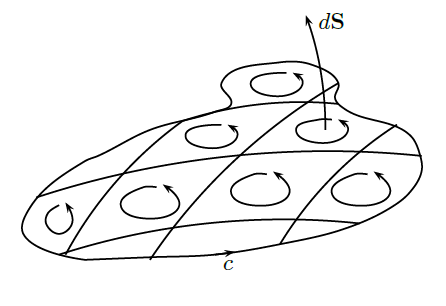
\includegraphics[scale=0.6]{Imagenes/Superficie_Elementos_Diferenciables.png}
    \caption{Descomposición de una superficie finita en elementos diferenciables.}
    \label{fig:figura_superficie_elementos_diferenciables}
\end{figure}
\end{frame}
\begin{frame}
\frametitle{Cálculos para una superficie abierta}
Los circuitos con lados comunes no contribuyen a la circulación.
\\
\bigskip
\pause
La contribución neta se debe solo a los elementos de línea ubicados en el contorno $c$.
\end{frame}
\begin{frame}
\frametitle{Teorema de Stokes}
Entonces tenemos:
\pause
\begin{align}
\scaleoint{6ex}_{c} \vb{B} \cdot \dd{\vb{l}} = \scaleint{6ex}_{\bs S} \curl{\vb{B}} \cdot \dd{\vb{S}}
\label{eq:ecuacion_01_35}
\end{align}
Que conocemos con el \emph{Teorema de Stokes}, que nos permite reemplazar integrales de área por integrales de línea.
\end{frame}
% \begin{frame}
% \frametitle{Ejercicio a cuenta}
% Demuestra que:
% \begin{align*}
% \curl(\phi \, \vb{A}) = \phi \, \curl{\vb{A}} + \grad{\phi} \times \vb{A}
% \end{align*}
% \end{frame}
\begin{frame}
\frametitle{Ejercicio a cuenta}
El campo electrostático de un dipolo eléctrico $\vb{p} = p_{0} \, \vu{e}_{z}$ es:
\begin{align*}
\vb{E} = \dfrac{p_{0} (2 \, \vb{e}_{r} \, \cos \theta + \vu{e}_{\theta} \, \sin \theta)}{r^{3}}
\end{align*}
Demuestra que:
\setbeamercolor{item projected}{bg=ao,fg=yellow}
\setbeamertemplate{enumerate items}{%
\usebeamercolor[bg]{item projected}%
\raisebox{1.5pt}{\colorbox{bg}{\color{fg}\footnotesize\insertenumlabel}}%
}
\begin{enumerate}
\item $\curl{\vb{E}} = 0$
\item para $r \neq 0$, se tiene $\div{\vb{E}} = 0$
\end{enumerate}
\end{frame}

\section{Laplaciano}
\frame[allowframebreaks]{\frametitle{Temas a revisar} \tableofcontents[currentsection, hideothersubsections]}
\subsection{Definición}

\begin{frame}
\frametitle{Definición del operador}
El Laplaciano de una función escalar $f(u_{i})$, que se representa por $\laplacian{f(u_{i})}$, se define como:
\pause
\begin{align*}
\laplacian{f} = \div{\nabla f}
\end{align*}
\end{frame}
\begin{frame}
\frametitle{Definición del operador}
Entonces por la ec. (\ref{eq:ecuacion_01_30}), con $B_{i} = (\nabla f)$:
\pause
\begin{align*}
\laplacian{f} = \dfrac{1}{h} \, \nsum_{i=1}^{3} \pdv{u_{i}} \left( \dfrac{h}{h_{i}}  (\nabla f)_{i} \right)
\end{align*}
con $h = h_{1} h_{2} h_{3}$
\\
\pause
De acuerdo con la ec. (\ref{eq:ecuacion_01_28}):
\pause
\begin{align*}
(\nabla f) = \dfrac{1}{h_{i}} \pdv{f}{u_{i}}
\end{align*}
\end{frame}
\begin{frame}
\frametitle{Definición del operador}
Se sigue entonces que:
\pause
\begin{align}
\laplacian{f} = \dfrac{1}{h} \, \nsum_{i=1}^{3} \pdv{u_{i}} \left( \dfrac{h}{h_{i}^{2}}  \pdv{f}{u_{i}} \right)
\label{eq:ecuacion_01_36}
\end{align}
\end{frame}

\subsection{Laplaciano en coordenadas ortogonales}

\begin{frame}
\frametitle{Laplaciano en coord. ortogonales}
El Laplaciano en coordenadas cartesianas:
\pause
donde $h_{x} = h_{y} = h_{z} = 1$:
\begin{align*}
\laplacian{f} &= \pdv[2]{f}{x} + \pdv[2]{f}{y} + \pdv[2]{f}{z}
\end{align*}
\end{frame}
\begin{frame}
\frametitle{Laplaciano en coord. ortogonales}
El Laplaciano en coordenadas cilíndricas:
\pause
donde:
\begin{align*}
h_{\rho} &= h_{z} = 1, \quad h_{\phi} = \rho \\
h &= \rho
\end{align*}
\pause
\vspace*{-0.5cm}
\begin{eqnarray*}
\begin{aligned}
\laplacian{f} &= \dfrac{1}{\rho} \pdv{\rho} \left( \dfrac{\rho}{1} \pdv{f}{\rho} \right) {+} \dfrac{1}{\rho} \pdv{\phi} \left( \dfrac{\rho}{\rho^{2}} \pdv{f}{\phi} \right) {+} \dfrac{1}{\rho} \pdv{z} \left( \dfrac{\rho}{1} \pdv{f}{z} \right) = \\[0.5em] \pause
&= \dfrac{1}{\rho} \, \pdv{\rho} \left( \rho \, \pdv{f}{\rho} \right) + \dfrac{1}{\rho^{2}} \, \pdv[2]{f}{\phi} + \pdv[2]{f}{z} 
\end{aligned}
\end{eqnarray*}
\end{frame}
\begin{frame}
\frametitle{Laplaciano en coord. ortogonales}
El Laplaciano en coordenadas esféricas con:
\begin{align*}
h_{r} = 1, \quad h_{\theta} = r, \quad h_{\varphi} = r \sin \theta \hspace{0.5cm} h = r^{2} \sin \theta
\end{align*}
\pause
\vspace*{-0.5cm}
\begin{align*}    
\laplacian{f} &= \dfrac{1}{r^{2}} \pdv{r} \left( r^{2} \pdv{f}{r} \right) + \dfrac{1}{r^{2} \sin \theta} \, \pdv{\theta} \left( \sin \theta \pdv{f}{\theta} \right) + \\[0.5em]
&+ \dfrac{1}{r^{2} \, \sin^{2} \theta} \, \pdv[2]{f}{\varphi}
\end{align*}
\end{frame}
\begin{frame}
\frametitle{Ejercicio a cuenta}
Usando coordenadas curvilíneas demuestra que:
\begin{align*}
\laplacian{(\phi \, \psi)} = \phi \, \laplacian{\psi} + \psi \, \laplacian{\phi} + 2 \, \grad{\phi} \vdot \grad{\psi}
\end{align*}
\end{frame}

\subsection*{Laplaciano de función vectorial}

\begin{frame}
\frametitle{Laplaciano de función vectorial}
En otros sistemas de coordenadas, el Laplaciano de una función vectorial se define por:
\pause
\begin{align*}
\laplacian{\vb{A}} = \grad{(\div{A})} - \curl{(\curl{\vb{A}})}
\end{align*}
\end{frame}

\subsection{El Laplaciano en la física}

\begin{frame}
\frametitle{El Laplaciano en la física}
El Laplaciano se encontrará en distintas áreas de la física: electrostática, magnetostática, gravitación, flujo de fluidos, mecánica cuántica, difusión de calor entre otros.
\end{frame}
\begin{frame}
\frametitle{Resultados importantes}
El tipo más sencillo de campo vectorial $\vb{F}(\vb{r})$ es donde el campo es irrotacional, incompresible (llamado también de divergencia nula), continuo y derivable.
\end{frame}
\begin{frame}
\frametitle{Campo irratocional}
Por ser un campo irrotacional, donde $\curl{\vb{F}} = 0$, existe un potencial $\phi$, tal que:
\pause
\begin{align*}
\vb{F} = \grad{\phi}
\end{align*}
\pause
Por ser un campo incompresible, donde $\div{\vb{F}} = 0$, entonces:
\pause
\begin{align*}
\laplacian{\phi} = 0
\end{align*}
\end{frame}
\begin{frame}
\frametitle{Soluciones armónicas}
La solución a la ecuación de Laplace se denomina \textocolor{darkmagenta}{función armónica}.
\\
\bigskip
\pause
El potencial de un campo electrostático es armónico en el exterior de las cargas; mientras que en un fluido de densidad constante, el potencial de velocidad es armónico, si no hay fuentes ni sumideros.
\end{frame}

\section{Utilidad de los operadores}
\frame[allowframebreaks]{\frametitle{Temas a revisar} \tableofcontents[currentsection, hideothersubsections]}
\subsection{Expresión de ecuaciones diferenciales}

\begin{frame}
\frametitle{Utilidad de los operadores}
Con la construcción que hemos revisado, ahora tenemos la oportunidad de expresar fenómenos físicos en algún sistema coordenado particular, de tal manera que si están involucrados los operadores diferenciales, la ecuación resultante será más fácil de manejar.
\end{frame}
\begin{frame}
\frametitle{Preparados para el Tema 2}
Una vez que hayamos expresado la ecuación diferencial, el siguiente paso será resolverla.
\\
\bigskip
\pause
Para ello, revisaremos algunas técnicas de solución que se trabajarán en el \emph{\textcolor{blue}{Tema 2 - Primeras técnicas de solución}}. Antes resolveremos algunos ejercicios.
\end{frame}
\end{document}